\documentclass[a4paper, 11pt]{article}
\usepackage[UTF8]{ctex}
\usepackage{amssymb}
\usepackage{amsmath}
\usepackage{graphicx}
\usepackage{geometry}
\usepackage{listings}
\usepackage{enumerate}
\usepackage{subfigure}
\usepackage{cases}
\usepackage[ruled,vlined]{algorithm2e}
\geometry{scale=0.8}
\usepackage{hyperref}
\usepackage{bookmark}
\linespread{1.5}

\title{
\normalfont \normalsize
\textsc{School of Data and Computer Science, Sun Yat-sen University} \\ [25pt] %textsc small capital letters
\rule{\textwidth}{0.5pt} \\[0.4cm] % Thin top horizontal rule
\huge  T04 Machine Learning\\ % The assignment title
\rule{\textwidth}{2pt} \\[0.5cm] % Thick bottom horizontal rule
\author{16337110 匡乾, 16337111 赖若潘}
\date{\normalsize\today}
}

\begin{document}
\maketitle
\tableofcontents
\newpage
\section{Q1}
\begin{enumerate}[(a)]
  \item
  \begin{itemize}
    \item 分裂前:Likes中true有5个,false有7个。
    \item 分裂后:Lawyers = true的6个数据中,
    Likes中true有4个,false有2个;\\
    Lawyers = false的6个数据中,Likes中true有1个,false有5个
  \end{itemize}
  $Remainder(Lawyers) = \frac{1}{2}B(\frac{2}{3}) + \frac{1}{2}B(\frac{1}{6})$\\
  $Gain(Lawyers) = B(\frac{5}{5+7}) - Remainder(Lawyers)$\\
  $= \frac{7}{12}log_2(\frac{12}{7})+
                \frac{5}{12}log_2(\frac{12}{5})-
                \frac{1}{2}[\frac{2}{3}log_2(\frac{3}{2})+\frac{1}{3}log_2(3)
                +\frac{1}{6}log_2(6)+\frac{5}{6}log_2(\frac{6}{5})]
                = 0.1957$
  \item
  第一次分裂同(a)所述,接下来继续对子树进行递归分裂。
  \begin{enumerate}[(1)]
    \item Laywers = true的节点中,在Comedy,Doctors,
    Guns选择最佳属性来分裂。\\
    $Gain(Laywers=true,Comedy) = B(\frac{2}{3})-
    \frac{1}{3}B(1)-\frac{2}{3}B(\frac{1}{2}) = 0.2516$\\
    $Gain(Laywers=true,Doctors) = B(\frac{2}{3})-
    \frac{1}{2}B(\frac{1}{3})-\frac{1}{2}B(\frac{1}{3}) = 0$\\
    $Gain(Laywers=true,Guns) = B(\frac{2}{3})-
    \frac{1}{3}B(1)-\frac{2}{3}B(\frac{1}{2}) = 0.2516$\\
    所以选择Gain最大的Comedy属性进行分裂。
      \begin{enumerate}
        \item Laywers = true且Comedy = true的节点中,
        因为所有数据都属于同一类(Likes=true),所以停止分裂。
        \item Laywers = true且Comedy = false的节点中,
        在Doctors,Guns选择最佳属性来分裂。\\
        $Gain(Laywers=true,Comedy=false,Doctors) = B(\frac{1}{2})-
        \frac{1}{2}B(\frac{1}{2})-\frac{1}{2}B(\frac{1}{2}) = 0$\\
        $Gain(Laywers=true,Comedy=false,Guns) = B(\frac{1}{2})-
        \frac{1}{2}B(1)-\frac{1}{2}B(1) = 1$\\
        所以选择Gain最大的Guns属性进行分裂。
        \begin{enumerate}
          \item Laywers = true且Comedy = false且Guns = true的节点中,
          因为所有数据都属于同一类(Likes=true),所以停止分裂。
          \item Laywers = true且Comedy = false且Guns = false的节点中,
          因为所有数据都属于同一类(Likes=false),所以停止分裂。
        \end{enumerate}
      \end{enumerate}
    \item Laywers = false的节点中,在Comedy,Doctors,Guns选择最佳属性来分裂。\\
    $Gain(Laywers=false,Comedy) = B(\frac{1}{6})-
    \frac{1}{2}B(1)-\frac{1}{2}B(\frac{1}{3}) = 0.1909$\\
    $Gain(Laywers=false,Doctors) = B(\frac{1}{6})-
    \frac{1}{3}B(1)-\frac{2}{3}B(\frac{1}{4}) = 0.1092$\\
    $Gain(Laywers=false,Guns) = B(\frac{1}{6})-
    \frac{1}{2}B(1)-\frac{1}{2}B(\frac{1}{3}) = 0.1909$\\
    所以选择Gain最大的Comedy属性进行分裂。

      \begin{enumerate}
        \item Laywers = false且Comedy = true的节点中,
        在Doctors,Guns选择最佳属性来分裂。\\
        $Gain(Laywers=false,Comedy=true,Doctors) = B(\frac{1}{3})-
        \frac{1}{3}B(0)-\frac{2}{3}B(\frac{1}{2}) = 0.2516$\\
        $Gain(Laywers=false,Comedy=true,Guns) = B(\frac{1}{3})-
        \frac{2}{3}B(1)-\frac{1}{3}B(1) = 0.9183$\\
        所以选择Gain最大的Guns属性进行分裂。
          \begin{enumerate}
            \item Laywers = false且Comedy = true且Guns = true的节点中,
            因为所有数据都属于同一类(Likes=false),所以停止分裂。
            \item Laywers = false且Comedy = true且Guns = false的节点中,
            因为所有数据都属于同一类(Likes=true),所以停止分裂。
          \end{enumerate}

        \item Laywers = false且Comedy = false的节点中,
        因为所有数据都属于同一类(Likes=false),所以停止分裂。
      \end{enumerate}
  \end{enumerate}
\end{enumerate}
决策树建立过程如图(\ref{fig:Q1})
\begin{figure}[ht]
  \centering
  \subfigure[分裂Lawyers]{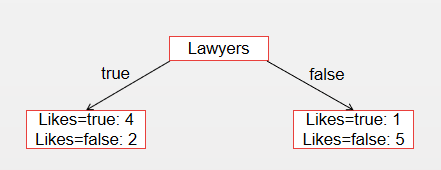
\includegraphics[width=0.4\columnwidth]{Q1-1.png}}
  \subfigure[Lawyers=true,分裂Comedy]{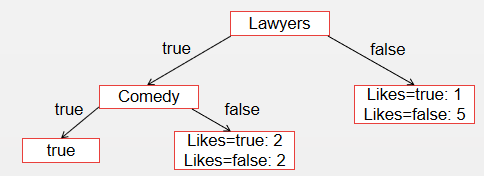
\includegraphics[width=0.4\columnwidth]{Q1-2.png}}
  \subfigure[Lawyers=true,Comedy=false,分裂Guns]{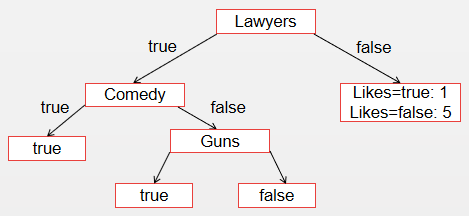
\includegraphics[width=0.4\columnwidth]{Q1-3.png}}
  \subfigure[Lawyers=false,分裂Comedy]{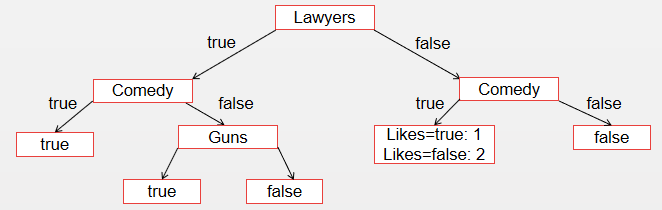
\includegraphics[width=0.5\columnwidth]{Q1-4.png}}
  \subfigure[Lawyers=false,Comedy=true,分裂Guns]{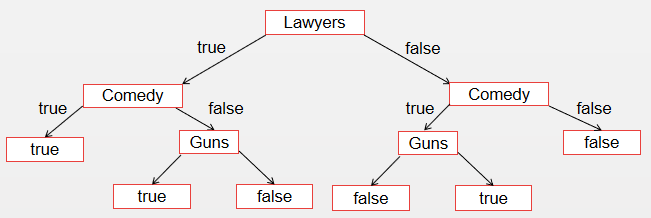
\includegraphics[width=0.6\columnwidth]{Q1-5.png}}
  \caption{决策树建立过程}
  \label{fig:Q1}
\end{figure}

\section{Q2}
h1: 100\% cherry

h2: 75\% cherry + 25\% lime

h3: 50\% cherry + 50\% lime

h4: 25\% cherry + 75\% lime

h5: 100\% lime

$d = [lime,cherry,cherry,lime,lime]$

$d' = [lime,cherry,lime,lime,lime]$

显然对于数据$d$和$d'$来说h1和h5是不可能的,因此只考虑h2,h3,h4

\begin{enumerate}[(a)]
\item

$\because$
$h_{MAP(d)} = argmax_h P(h)P(d|h)$
$$\begin{cases}
	P(h_2)P(d|h_2) = 0.2 * C_5^2 (\frac{3}{4})^2 (\frac{1}{4})^3 = \frac{18}{2^{10}}\\
	P(h_3)P(d|h_3) = 0.4 * C_5^2 (\frac{1}{2})^2 (\frac{1}{2})^3 = \frac{128}{2^{10}}\\
	P(h_4)P(d|h_4) = 0.2 * C_5^2 (\frac{1}{4})^2 (\frac{3}{4})^3 = \frac{54}{2^{10}}
\end{cases}$$
$\therefore h_{MAP(d)} = h_3$



$\because$
$h_{MAP(d')} = argmax_h P(h)P(d'|h)$
$$\begin{cases}
	P(h_2)P(d'|h_2) = 0.2 * C_5^1 (\frac{3}{4})^1 (\frac{1}{4})^4 = \frac{3}{2^{10}}\\
	P(h_3)P(d'|h_3) = 0.4 * C_5^1 (\frac{1}{2})^1 (\frac{1}{2})^4 = \frac{64}{2^{10}}\\
	P(h_4)P(d'|h_4) = 0.2 * C_5^1 (\frac{1}{4})^1 (\frac{3}{4})^4 = \frac{81}{2^{10}}
\end{cases}$$\\
$\therefore h_{MAP(d')} = h_4$


由题意知,$h_{MAP} = h_3 = h_{MAP(d)}$,故遗失的数据应该为cherry。

\item
Bayesian Learning:\\
$\because$
$P(X|d) = \sum_{i} P(X|h_i) P(h_i|d)
		= \sum_{i} P(X|h_i) \alpha P(d|h_i) P(h_i)$\\
$\therefore$$P(lime|d) - P(cherry|d)\\
= (P(lime|h_2)-P(cherry|h_2)) \alpha P(d|h_2) P(h_2) + (P(lime|h_3)-P(cherry|h_3)) \alpha P(d|h_3) P(h_3) + (P(lime|h_4)-P(cherry|h_4)) \alpha P(d|h_4) P(h_4) \\
= 0.5 * \alpha (P(d|h_4) P(h_4) - P(d|h_2) P(h_2))\\
= 0.5 * \alpha * \frac{36}{2^{10}}\\
> 0$

$\therefore$
第六个candy应该是lime口味的。

ML Learning:\\
$h_{ML} = argmax_h P(d|h)$\\
显然h1和h5依然是不可能的
$$\begin{cases}
	P(d|h_2) = C_5^2 (\frac{3}{4})^2 (\frac{1}{4})^3 = \frac{90}{2^{10}}\\
	P(d|h_3) = C_5^2 (\frac{1}{2})^2 (\frac{1}{2})^3 = \frac{320}{2^{10}}\\
	P(d|h_4) = C_5^2 (\frac{1}{4})^2 (\frac{3}{4})^3 = \frac{270}{2^{10}}
\end{cases}$$
$\therefore h_{ML} = h_3$\\
$\because P(cherry|h_3) = 0.5 = P(lime|h_3)$\\
$\therefore$故无法确定第六个糖果的口味(lime和candy的可能性相同)
\end{enumerate}

\section{Q3}

\IncMargin{1em}
\begin{algorithm}[H]
\SetKwInOut{Input}{Input}
\SetKwInOut{Output}{Output}
\SetKwInOut{Local}{Local}
\Input{
  X set of features X = $\{ X_1,...,X_{n}\}$\\
  D data set on features $\{ X_1,...,X_{n}\}$\\
  k number of classes
}
\Output{
  $P(C),P(X_i|C)$ for each i $\in \{ 1:n\}$,
  where C = $\{ 1,...,k\}.$
}
\Local{
  real array $P\big[C\big]$\\
  real arrays $M_i \big[X_i,C\big]$
  for each i $\in \{ 1:n\}$\\
  real arrays $P_i \big[X_i,C\big]$
  for each i $\in \{ 1:n\}$
}
\BlankLine
s := number of tuples in D\\
Assign $P\big[C\big],P_i \big[X_i,C\big]$ arbitrarily\\
\Repeat{termination}
{
  Assign $M_i \big[X_i,C\big]\ to\ all\ 0,i \in \{ 1:n\}$\\
  \BlankLine
  \For{each assignment $\langle
  X_1 = v_1,...,X_n = v_n\rangle \in D$}
  {
    let $m \leftarrow |\langle
    X_1 = v_1,...,X_n = v_n\rangle \in D|$\\
    \For{each $c \in \{ 1:k\}$}
    {
      \For{each $i \in \{ 1:k\}$}
      {
        $M_i \big[X_i=v_i,C=c\big]\ +\!= m \times
        P(C=c|X_1 = v_1,...,X_i=v_i,...,X_n = v_n)$\\
      }
    }
  }
  \BlankLine
  \For{each $i \in \{ 1:k\}$}
  {
    $P_i \big[X_i,C\big] = \frac{M_i[X_i,C]}{\sum_{C}M_i[X_i,C]}$
  }
  \BlankLine
  $P\big[C\big] = \sum_{X_1}M_1\big[X_1,C\big]/s$
}
\caption{EM(X,D,k)}
\label{EM}
\end{algorithm}\DecMargin{1em}

\section{Q4}
\begin{enumerate}[(a)]
\item
~\\
首先,由正项级数中“p级数”可知:\\
对于$\sum\limits _{n=1}^\infty \frac{1}{n^p}$,当$p>1$时收敛,当$p \leq 1$时发散,证明如下:\\
\begin{itemize}
  \item 当$p=1$时:设$2^k \leq n < 2^{k+1}$
  \begin{align*}
    S_n &= 1 + \frac{1}{2} + \frac{1}{3} + \cdots + \frac{1}{n} \\
    &= 1 + \frac{1}{2} + (\frac{1}{3} + \frac{1}{4}) + \cdots +
    (\frac{1}{2^{k-1}+1} + \frac{1}{2^{k-1}+2} + \cdots + \frac{1}{2^{k-1}+2^{k-1}})
    + \frac{1}{2^{k}+1} + \cdots + \frac{1}{n} \\
    &\ge \frac{1}{2} + \frac{1}{2} + (\frac{1}{4} + \frac{1}{4}) + \cdots + (\frac{1}{2^k} * 2^{k-1})  \\
    &= \frac{k+1}{2}
  \end{align*}
  此时k可以取任意大,因而$S_n$无上界。故$p=1$时,级数$\sum\limits _{n=1}^\infty \frac{1}{n}$发散。
  \item 当$p<1$时:对任意正整数k,有
  $$\frac{1}{k^p} \ge \frac{1}{k}$$
  $\therefore$
  $$\sum\limits _{k=1}^\infty \frac{1}{k^p} \ge \sum\limits _{k=1}^\infty \frac{1}{k}$$
  右边部分数列无上界故左边也无上界,故$\sum\limits _{n=1}^\infty \frac{1}{n^p}$在$p<1$也发散
  \item 当$p>1$时:设$2^k \leq n < 2^{k+1}$
  \begin{align*}
    S_n &= 1 + \frac{1}{2^p} + \frac{1}{3^p} + \cdots + \frac{1}{n^p} \\
    &= 1 + (\frac{1}{2^p} + \frac{1}{3^p})  + \cdots +
    [\frac{1}{(2^{k-1})^p} + \frac{1}{(2^{k-1}+1)^p} + \cdots + \frac{1}{(2^{k}-1)^p}]
    + \frac{1}{(2^k)^p}  + \cdots + \frac{1}{n^p} \\
    &\leq 1 + \frac{2}{2^p} + \frac{4}{4^p} + \cdots + \frac{2^{k-1}}{(2^{k-1})^p} + \frac{2^k}{(2^k)^p} \\
    &= 1 + \frac{1}{2^{p-1}} + (\frac{1}{2^{p-1}})^2 + \cdots + (\frac{1}{2^{p-1}})^{k-1} + + (\frac{1}{2^{p-1}})^{k} \\
    &= \frac{1-(\frac{1}{2^{p-1}})^{k+1}}{1-\frac{1}{2^{p-1}}} \\
    &\leq \frac{1}{1-\frac{1}{2^{p-1}}} \\
    &= \frac{2^{p-1}}{2^{p-1}+1}
  \end{align*}
  因此部分和数列有上界,故$\sum\limits _{n=1}^\infty \frac{1}{n^p}$当$p>1$时收敛
\end{itemize}
其次,Convergence can be guaranteed if $\sum\limits _{k=1}^\infty \alpha_k = \infty$ and $\sum\limits_{k=1}^\infty \alpha_k^2 < \infty$\\

$\therefore$
\begin{itemize}
  \item 当$\alpha_k = 1/k$时:\\
  由正项级数中“p级数”可知,$\sum\limits _{k=1}^\infty \alpha_k = \infty \ (p=1)$ 而且 $\sum\limits_{k=1}^\infty \alpha_k^2 < \infty \ (p=2)$,满足收敛条件
  \item 当$\alpha_k = 10/(9+k)$时:\\
  由正项级数中“p级数”以及比较判别法的极限形式可知,$\sum\limits _{k=1}^\infty \alpha_k = \infty \ (p=1)$ 而且 $\sum\limits_{k=1}^\infty \alpha_k^2 < \infty \ (p=2)$,满足收敛条件
  \item 当$\alpha_k = 0.1$时:\\
  因为$\sum\limits_{k=1}^\infty \alpha_k^2 = \lim\limits_{x \rightarrow \infty} 0.01*x = \infty $,故不满足收敛条件
  \item 当$\alpha_k = 0.1,0.01,0.001...$时:\\
  \begin{align*}
    \sum\limits _{k=1}^\infty \alpha_k &= 1000 + 100 + 10 + \cdots \\
    &= \sum\limits _{n=1}^\infty 10000*(\frac{1}{10})^n \\
    &\leq \frac{1000}{1-\frac{1}{10}} \\
    &< \infty
  \end{align*}
  故$\sum\limits _{k=1}^\infty \alpha_k < \infty$,不满足收敛条件
\end{itemize}
综上$\alpha_k = 1/k$以及$\alpha_k = 10/(9+k)$时有$\sum\limits _{k=1}^\infty \alpha_k = \infty$ 和 $\sum\limits_{k=1}^\infty \alpha_k^2 < \infty$,满足收敛条件。

\item
使用了帅哥TA提供的E14中的Q-learning样例(见图Q4-b)\\
\begin{figure}[h]
	\centering
	\includegraphics[scale = 0.28]{Q4-B.png}
  \caption{Q4-b}
\end{figure}

保持learning rate = 0.8 不变,episode分别取10000和100000,显然第一个和第二个$\alpha_k$此时都还没收敛,而第三个和第四个$\alpha_k$已经收敛了。经检验,在9000左右时,第三个和第四个$\alpha_k$完成收敛到真实Q-Value(因为在$k < 10000$时,第三个和第四个$\alpha_k$有相同的取值,故为同时收敛的)\\
当然对于不同的域来说,其结果是不同的。首先第一个条件$\sum\limits _{k=1}^\infty \alpha_k = \infty$确保了随机函数和初始条件排除了平均值的情况,第二个条件$\sum\limits_{k=1}^\infty \alpha_k^2 < \infty$保证收敛性,因此在不同域的情况下,第三个和第四个$\alpha_k$不一定能确保收敛,但在k不够大的情况下,第一个和第二个$\alpha_k$同样也不能确保收敛。
\item
我认为environment adapts slowly意思是learning rate较小,因此learning rate分别取0.1和0.01的情况下,$\alpha_k = 10/(9+k)$的表现有很大的改进,它可以更快的收敛,大概在100000次时已经收敛到真实Q-Value。

% $\because$
% $Q[s,a] \leftarrow (1-\alpha)Q[s,a] + \alpha(r+\gamma max_{a'}Q[s',a'])$
% $Q[s,a] \leftarrow Q[s,a] + \alpha(r+\gamma max_{a'}Q[s',a']-Q[s,a])$
\end{enumerate}



%\clearpage
%\bibliography{E:/Papers/LiuLab}
%\bibliographystyle{apalike}
\end{document}


%%% Local Variables:
%%% mode: latex
%%% TeX-master: t
%%% End:
